\chapter{Análisis del Software}

En este capítulo, se desarrollan los aspectos necesarios para la definición del
proceso de desarrollo del \emph{framework}, primeramente se hará referencia a
las cuestiones relacionadas con las fuentes de análisis utilizadas, y algunos
conceptos puntuales acerca del producto, y la descripción de las actividades
planificadas durante el proyecto.

Posteriormente se describirán los \emph{tours} realizados en el sistema como
parte del análisis de los elementos, los cálculos de valor limite realizados
sobre los formularios, para terminar condensando los casos de prueba
formulados.

\section{Entorno de proyecto}
Los primeros componentes que se describirán son los relacionados con el entorno
del proyecto, que son aquellos factores del contexto que incluyen recursos
necesarios, restricciones, y cualquier otro elemento del proyecto que debe ser
tomado en cuenta para la evaluación.

\subsection{Fuentes de Información}
Para evaluar los componentes definidos en el proyecto, se encontraron
y recurrirán a las siguientes fuentes de información respecto al producto:

\begin{description}
\item [Centro de Ayuda] \emph{Salesforce} ofrece un amplio conjunto de
documentación, información general, preguntas frecuentes, y contacto con el
servicio de asistencia técnica desde su sitio de ayuda
(\emph{https://help.salesforce.com/}).

Estos recursos serán útiles para conocer los reclamos de los usuarios, las
características criticas del producto, y las estrategias del fabricante hacia
sus clientes.

\item [Centro de Desarrollo] \emph{Salesforce} también posee un sitio web
específicamente para compartir recursos de desarrollo sobre la plataforma
(\emph{https://developer.salesforce.com/}).

Este sitio se podrá aprovechar para consultar las referencias a las \emph{API}
del servicio, conocer las posibilidades que proveen los componentes y como
pueden aprovecharse desde la perspectiva del desarrollador.

\item [Recursos para administradores] Sitio web enfocado a ofrecer experiencias,
vídeos, herramientas, y un sin fin de recursos orientados a usuarios con un rol
administrativo de recursos sobre la plataforma
(\emph{https://admin.salesforce.com/resources}).

Este sitio será útil para entender las diferencias existentes entre la
funcionalidad provista a un usuario normal y a otro administrador, además de
conocer los permisos y roles de usuario en profundo.

\item [Comunidad \emph{Trailblazer}] Sitio web enfocado a conectar a miembros de
la comunidad \emph{Salesforce}, para compartir experiencias, aprender, y proveer
de nuevas ideas sobre la utilización del servicio
(\emph{https://success.salesforce.com/}).

Este sitio también sirve como fuente de reclamos de los usuarios,
funcionalidades criticas, y errores comunes encontrados en el servicio.

\end{description}

\subsection{\emph{Salesforce}}
\emph{Salesforce} cuenta con múltiples ediciones que comparten una apariencia,
pero varían según la funcionalidad y los costos del servicio. Según la
documentación del fabricante algunos clientes comienzan con una edición básica y
actualizan a una edición más rica en características a medida que evolucionan
los requisitos empresariales.

En el \emph{cuadro \ref{ediciones}} se describen las ediciones disponibles con
las que cuenta el servicio actualmente, cabe comentar que la evaluación se
realizará sobre la versión \emph{Developer} debido a que está es la que requiere
para su utilización, la menor cantidad de restricciones de parte del fabricante.

\begin{table}
\centering
\begin{tabular}{|l|p{12.0cm}|}
\hline
\footnotesize{\textbf{Edición}} & \footnotesize{\textbf{Descripción}} \\
\hline
\footnotesize{\emph{Essentials}} & \footnotesize{Diseñado para pequeños negocios
para empezar a trabajar con un sistema de \emph{CRM} de forma rápida. Incluye
presentaciones interactivas y un asistente de configuración para comenzar, una
interfaz de usuario fácil de utilizar y herramientas de administración para
personalizar su implementación conforme crece.} \\
\footnotesize{\emph{Professional}} & \footnotesize{Diseñado para negocios que
requieren la funcionalidad completa de \emph{CRM}. Incluye herramientas de
personalización, integración y administración directas y fáciles de usar para
facilitar cualquier implementación de pequeño y mediano tamaño.} \\
\footnotesize{\emph{Enterprise}} & \footnotesize{Cumple las necesidades
comerciales grandes y complejas. Proporciona herramientas avanzadas de
personalización y administración, además de todas las funcionalidades
disponibles en \emph{Professional Edition}, que pueden admitir implementaciones
a gran escala. \emph{Enterprise Edition} también incluye acceso a las \emph{API}
de \emph{Salesforce} para que pueda integrar fácilmente sistemas de gestión
interna.} \\
\footnotesize{\emph{Unlimited}} & \footnotesize{Proporciona nuevos niveles de
flexibilidad de plataforma para gestionar y compartir toda su información según
demanda. Incluye todas las funcionalidades de \emph{Enterprise Edition} además
de \emph{Premier Support}, acceso móvil completo, aplicaciones personalizadas
sin límite, límites de almacenamiento ampliados y otras funciones.} \\
\footnotesize{\emph{Developer}} & \footnotesize{Proporciona acceso a las
\emph{API} y la plataforma \emph{Lightning}. Permite a los desarrolladores
ampliar \emph{Salesforce}, integrarlo con otras aplicaciones y desarrollar
nuevas herramientas y aplicaciones. \emph{Developer Edition} ofrece además
acceso a muchas de las funciones disponibles en \emph{Enterprise Edition.}} \\
\hline
\end{tabular}
\caption{Ediciones actualmente disponibles de \emph{Sales Cloud}.}
\label{ediciones}
\source{https://help.salesforce.com/articleView?id=overview\_edition.htm}
\end{table}

Otra característica actual de \emph{Salesforce} es que cuenta con dos interfaces
web diferentes: la antigua conocida como: \emph{Salesforce Classic}, y la nueva
incluida desde 2015 denominada: \emph{Salesforce Lightning}; que tiene como
objetivo principal la unificación del comportamiento y la apariencia a través de
todo el servicio sea cual sea el dispositivo que el cliente
utilice \parencite{McCarthy}.

Se evaluarán las funcionalidades de los módulos sobre el navegador cuya
participación en el mercado es la mayor, en este caso: \emph{Google Chrome}
como puede verse en la \emph{figura \ref{software}}, priorizando las pruebas
sobre resoluciones de pantalla no menores a 1024 píxeles por 768 píxeles.

\begin{figure}
\centering
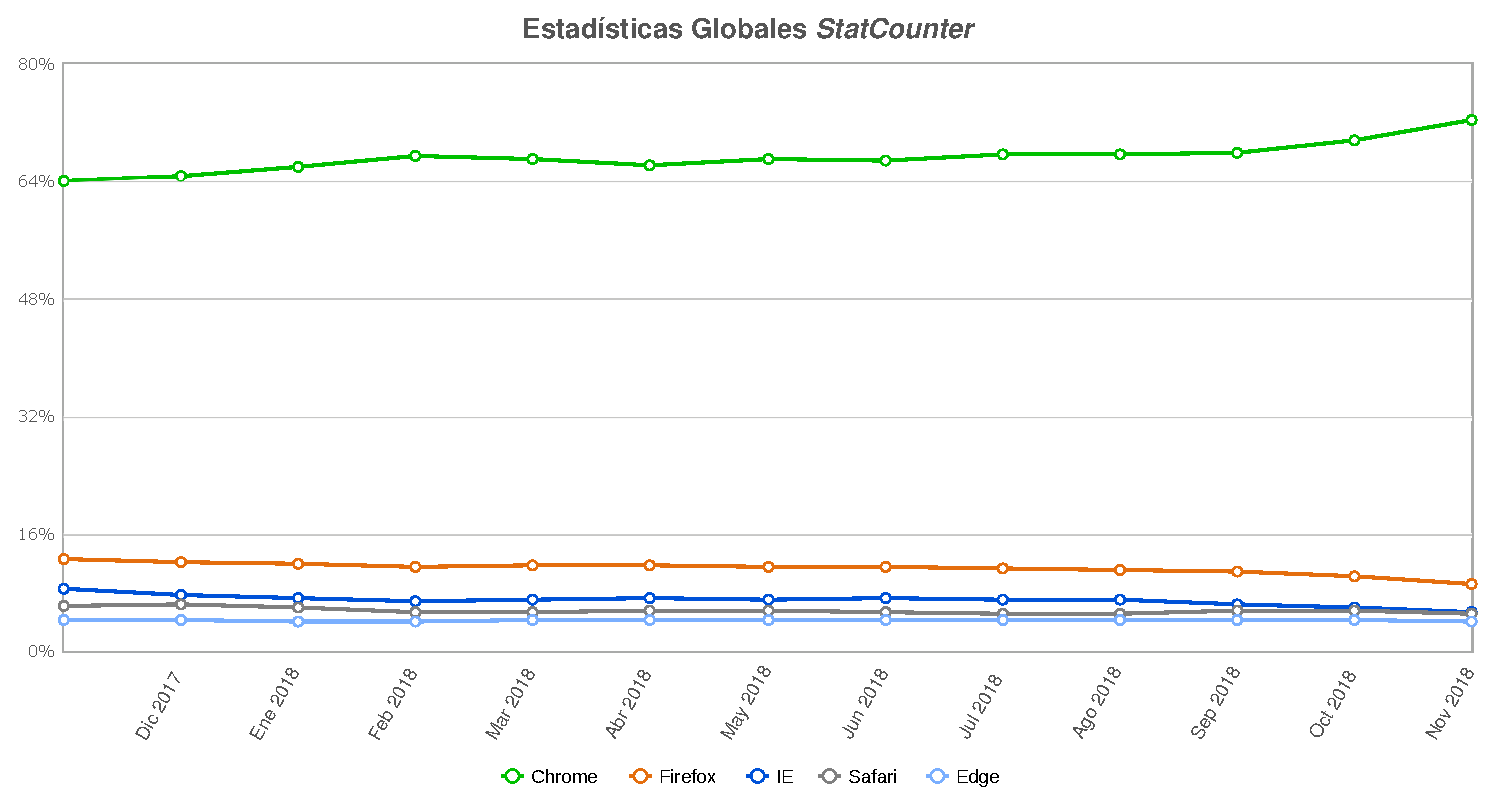
\includegraphics[width=1.0\textwidth]{graphics/compatibilidad.eps}
\caption{Participación de mercado de los navegadores hasta Noviembre del 2018.}
\label{software}
\source{http://gs.statcounter.com/browser-market-share/desktop/worldwide}
\end{figure}

Adicionalmente al uso del navegador \emph{Google Chrome} serán necesarios
otros navegadores para realizar la evaluación de compatibilidad sobre
vistas especificas del sistema, para este fin se consultó la información
disponible en la pagina de soporte provista por el fabricante, la cual como
puede verse en el \emph{cuadro \ref{soporte_navegadores}}, revela que se
soportan cinco navegadores diferentes bajo condiciones de limitación descritas
por el fabricante.

\begin{table}
\centering
\begin{tabular}{|p{6.0cm}|p{2.5cm}|p{1.4cm}|p{1.3cm}|p{1.3cm}|p{1.0cm}|}
\hline
& \footnotesize{\textbf{\emph{Microsoft Internet Explorer}}}
& \footnotesize{\textbf{\emph{Microsoft Edge}}}
& \footnotesize{\textbf{\emph{Google Chrome}}}
& \footnotesize{\textbf{\emph{Mozilla Firefox}}}
& \footnotesize{\textbf{\emph{Apple Safari}}} \\
\hline
\footnotesize{\emph{Lightning Experience}}
& \footnotesize{IE11 (EOL Diciembre 31, 2020)}
& \footnotesize{Ultima versión}
& \footnotesize{Ultima versión}
& \footnotesize{Ultima versión}
& \footnotesize{11.x+} \\
\footnotesize{\emph{Lightning Communities}}
& \footnotesize{IE11 (EOL Diciembre 31, 2020)}
& \footnotesize{Ultima versión}
& \footnotesize{Ultima versión}
& \footnotesize{Ultima versión}
& \footnotesize{11.x+} \\
\footnotesize{¿Consideraciones especiales de configuración?}
& \footnotesize{No}
& \footnotesize{No}
& \footnotesize{No}
& \footnotesize{No}
& \footnotesize{No} \\
\footnotesize{Limitaciones conocidas}
& \footnotesize{Sí}
& \footnotesize{Si}
& \footnotesize{No}
& \footnotesize{Si}
& \footnotesize{Si} \\
\hline
\end{tabular}
\caption{Lista de compatibilidad provista por \emph{Salesforce}.}
\label{soporte_navegadores}
\source{https://help.salesforce.com/articleView?id=getstart\_browsers\_sfx.htm}
\end{table}

\section{Planificación de actividades}
Para conseguir los objetivos planteados por el proyecto se realizarán las
actividades detalladas en el \emph{cuadro \ref{planificacion}} en la página
\pageref{planificacion}. Este cuadro detalla las actividades agrupadas por el
objetivo especifico y detallando también el resultado esperado de estas.

\begin{sidewaystable}
\renewcommand{\arraystretch}{1}
\linespread{1.25}
\centering
\small
\begin{tabular}{|l|l|p{6.5cm}|l|}
\hline
Objetivo General & Objetivos Específicos & Actividades & Resultados \\
\hline
\multirow{10}{4.0cm}{Implementar un \emph{framework} para la automatización de
las pruebas de interfaz de usuario en el módulo de Productos y Listas de Precios
en \emph{Salesforce}, para garantizar un procedimiento continuo de evaluación y
minimizar la cantidad de errores que contiene el software.} &
\multirow{3}{4.0cm}{Formular los casos de prueba necesarios que los módulos de
gestión de productos y listas de precios requieran para cubrir los atributos de
calidad requeridos.} &
Recolección de la información y exploración de los módulos específicos. &
\multirow{3}{4.0cm}{Casos de prueba para los módulos de Productos y Listas de
Precios.} \\
\cline{3-3}
& & Análisis y diseño de los tipos de evaluación requeridos para los módulos
específicos. & \\
\cline{3-3}
& & Formulación los casos de prueba necesarios para los módulos
específicos. & \\
\cline{2-4}
& \multirow{3}{4.0cm}{Diseñar e implementar los modelos y bibliotecas de
funciones que conforman un \emph{framework} de automatización.} &
Análisis y modelamiento de los componentes del \emph{framework}. &
\multirow{3}{4.0cm}{\emph{Framework} de automatización con los componentes
necesarios para la implementación de los casos de prueba.} \\
\cline{3-3}
& & Estructuración de los entornos de prueba y configuración de los servicios
disponibles. & \\
\cline{3-3}
& & Implementación de los componentes del \emph{framework}. & \\
\cline{2-4}
& \multirow{4}{4.0cm}{Automatizar los casos de prueba de las funciones que
componen la interfaz de usuario del módulo de gestión de productos y listas de
precios.} &
Implementación de los casos de prueba formulados. &
\multirow{4}{4.0cm}{Rutinas de automatización de los casos de prueba de los
módulos de Productos y Listas de Precios.} \\
\cline{3-3}
& & Implementación de precondiciones y postcondiciones en la ejecución de los
casos de prueba. & \\
\cline{3-3}
& & Ejecución de los casos de prueba automatizados. & \\
\cline{3-3}
& & Generación del reporte de resultados y reporte de errores. & \\
\hline
\end{tabular}
\caption{Planificación de actividades del proyecto.}
\label{planificacion}
\source{Elaboración propia.}
\end{sidewaystable}

\section{Elementos del producto}
Dentro del alcance de la evaluación se encuentran los componentes de productos
y listas de precios, las funcionalidades que comprenden estos se detallan en
esta sección, desde múltiples perspectivas de análisis.

Como se mencionó anteriormente, se consideró la interfaz
\emph{Lightning Experience}, como único objetivo de la evaluación. La versión
\emph{Lightning Experience} esta disponible para las siguientes ediciones del
producto: \emph{Essentials}, \emph{Group}, \emph{Professional},
\emph{Enterprise}, \emph{Performance}, \emph{Unlimited}, y \emph{Developer}.

\subsection{Productos}
El Producto para el software a evaluar, representa uno de los componentes
fundamentales y claves para el éxito, por ende es importante evaluarlo
desde múltiples facetas; la primera de estas es la funcionalidad provista por
las interfaces de este módulo. En la \emph{figura \ref{productos}} pueden verse
estas funcionalidades, clasificadas desde la perspectiva de la interfaz de
usuario.

Entre las funcionalidades que pueden apreciarse están las operaciones comunes
de creación, búsqueda, visualización, modificación, y eliminación de productos,
se omitieron las funcionalidades de controles de vista de lista, para que
todo este componente pueda ser tratado de manera separada. También pueden
observarse funciones relacionadas a registrar precios estándar y precios para
una lista de precios determinada.

En la \emph{figura \ref{productos_vistas}}, se aprecian las diferentes vistas
que comprenden el módulo, se resaltaron las vistas que son de tipo formulario,
y también las que son de tipo confirmación de acción.

Además de las funcionalidades y vistas antes mencionadas, también se analizó el
comportamiento de los formularios que provee el módulo, como puede verse en la
\emph{figura \ref{productos_formularios}}.

\begin{figure}
\centering
\begin{tikzpicture}[
    grow via three points={one child at (0.5,-0.7) and
    two children at (0.5,-0.7) and (0.5,-1.4)},
    edge from parent path={(\tikzparentnode.south) |- (\tikzchildnode.west)}]
    \node {Productos}
        child { node {Nuevo}}
        child { node {Buscar: Producto}}
        child { node {Controles de Vista de Lista}
            child { node {\ldots}}
        }
        child [missing] {}
        child { node {Mostrar como}}
        child { node {Actualizar}}
        child { node {Filtrar por: Vista de Lista}}
        child { node {Modificar Lista}}
        child { node {Lista de Productos}
            child { node {Ver: Producto}
                child { node {Modificar}}
                child { node {Eliminar}}
                child { node {Duplicar}}
                child { node {Relacionado}
                    child { node {Agregar precio estándar}}
                    child { node {Agregar a lista de precios}}
                    child { node {Ver: Lista de precios}}
                    child { node {Modificar: Lista de precios}}
                    child { node {Eliminar: Lista de precios}}
                    child { node {Ver todos}
                        child { node {Actualizar}}
                    }
                }
                child [missing] {}
                child [missing] {}
                child [missing] {}
                child [missing] {}
                child [missing] {}
                child [missing] {}
                child [missing] {}
                child { node {Detalles}}
            }
            child [missing] {}
            child [missing] {}
            child [missing] {}
            child [missing] {}
            child [missing] {}
            child [missing] {}
            child [missing] {}
            child [missing] {}
            child [missing] {}
            child [missing] {}
            child [missing] {}
            child [missing] {}
            child { node {Modificar: Producto}}
            child { node {Eliminar: Producto}}
        };
\end{tikzpicture}
\caption{Funciones que componen el módulo de gestión de productos.}
\label{productos}
\source{Elaboración propia.}
\end{figure}

\begin{figure}
\centering
\begin{tikzpicture}[
    grow via three points={one child at (0.5,-0.7) and
    two children at (0.5,-0.7) and (0.5,-1.4)},
    edge from parent path={(\tikzparentnode.south) |- (\tikzchildnode.west)}]
    \node {Productos}
        child { node {Mostrar como}
            child { node {Tabla}}
            child { node {Kanban}}
        }
        child [missing] {}
        child [missing] {}
        child [missing] {}
        child { node [align=center] {<<\emph{formulario}>> \\ Crear Producto}}
        child [missing] {}
        child { node {Filtros}}
        child { node {Producto}
            child [missing] {}
            child { node [align=center] {<<\emph{formulario}>> \\ Modificar: Producto}}
            child [missing] {}
            child { node [align=center] {<<\emph{confirmación}>> \\ Eliminar: Producto}}
            child [missing] {}
            child { node [align=center] {<<\emph{formulario}>> \\ Crear Producto}}
            child [missing] {}
            child { node {Detalles}}
            child { node {Relacionado}
                child [missing] {}
                child { node [align=center] {<<\emph{formulario}>> \\ Crear Entrada del catalogo de precios}}
                child [missing] {}
                child { node [align=center] {<<\emph{formulario}>> \\ Agregar a lista de precios}}
                child [missing] {}
                child { node {Listas de precios}
                    child [missing] {}
                    child { node [align=center] {<<\emph{formulario}>> \\ Modificar Entrada del catalogo de precios}}
                    child [missing] {}
                    child { node [align=center] {<<\emph{confirmación}>> \\ Eliminar entrada del catalogo de precios}}
                    child [missing] {}
                }
            }
        }
        child [missing] {}
        child [missing] {}
        child [missing] {}
        child [missing] {}
        child [missing] {}
        child [missing] {}
        child [missing] {}
        child [missing] {}
        child [missing] {}
        child [missing] {}
        child [missing] {}
        child [missing] {}
        child [missing] {}
        child [missing] {}
        child [missing] {}
        child [missing] {}
        child { node [align=center] {<<\emph{formulario}>> \\ Modificar: Producto}}
        child [missing] {}
        child { node [align=center] {<<\emph{confirmación}>> \\ Eliminar: Producto}};
\end{tikzpicture}
\caption{Vistas que componen el módulo de gestión de productos.}
\label{productos_vistas}
\source{Elaboración propia.}
\end{figure}

\begin{figure}
\centering
\begin{tikzpicture}[
    grow via three points={one child at (0.5,-0.7) and
    two children at (0.5,-0.7) and (0.5,-1.4)},
    edge from parent path={(\tikzparentnode.south) |- (\tikzchildnode.west)}]
    \node {Productos}
        child [missing] {}
        child { node {Crear producto}
            child { node {Nombre del producto (*)}}
            child { node {Activo}}
            child { node {Código de producto}}
            child { node {Familia de productos}}
            child { node {Descripción del producto}}
        }
        child [missing] {}
        child [missing] {}
        child [missing] {}
        child [missing] {}
        child [missing] {}
        child [missing] {}
        child { node {Crear entrada del catálogo de precios}
            child { node {Producto (*)}}
            child { node {Activo}}
            child { node {Lista de precios (*)}}
            child { node {Precio de la lista (*)}}
            child { node {Utilizar precio estándar}}
        }
        child [missing] {}
        child [missing] {}
        child [missing] {}
        child [missing] {}
        child [missing] {}
        child [missing] {}
        child { node {Agregar a lista de precios}
            child { node {Lista de precios (*)}}
            child { node {Divisa (*)}}
        }
        child [missing] {}
        child [missing] {}
        child [missing] {}
        child { node {Modificar entrada del catálogo de precios}
            child { node {Activo}}
            child { node {Precio de la lista (*)}}
            child { node {Utilizar precio estándar}}
        };
\end{tikzpicture}
\caption{Formularios que componen el módulo de gestión de productos.}
\label{productos_formularios}
\source{Elaboración propia.}
\end{figure}

\subsection{Listas de Precios}
Las Listas de Precios, tienen como objetivo, hacer que un mismo producto pueda
tener múltiples precios, dependiendo de como la organización cliente maneje sus
canales de distribución y producción. Al igual que en el módulo de productos, en
la \emph{figura \ref{listas_de_precios}} pueden verse las funcionalidades
clasificadas desde la perspectiva de la interfaz de usuario, también se omitió
la sección de los controles de vista de lista.

Las funciones de Listas de Precios son muy similares a aquellas vistas en el
módulo de productos, analizado anteriormente.

En la \emph{figura \ref{listas_de_precios_vistas}}, se detallan aquellas vistas
presentes en este módulo, de la misma manera se ha destacado aquellas vistas que
son formularios, y aquellas que representan diálogos de confirmación.

También de las funcionalidades y vistas antes mencionadas, se analizó el
comportamiento de los formularios que provee este módulo, como puede verse en la
\emph{figura \ref{listas_de_precios_formularios}}.

\begin{figure}
\centering
\begin{tikzpicture}[
    grow via three points={one child at (0.5,-0.7) and
    two children at (0.5,-0.7) and (0.5,-1.4)},
    edge from parent path={(\tikzparentnode.south) |- (\tikzchildnode.west)}]
    \node {Listas de Precios}
        child { node {Nuevo}}
        child { node {Buscar: Lista de precios}}
        child { node {Controles de Vista de Lista}
            child { node {\ldots}}
        }
        child [missing] {}
        child { node {Mostrar como}}
        child { node {Actualizar}}
        child { node {Filtrar por: Vista de Lista}}
        child { node {Modificar Lista}}
        child { node {Lista de Listas de Precios}
            child { node {Ver: Lista de precios}
                child { node {Modificar}}
                child { node {Eliminar}}
                child { node {Duplicar}}
                child { node {Relacionado}
                    child { node {Agregar productos}}
                    child { node {Ver: Producto}}
                    child { node {Modificar: Producto}}
                    child { node {Eliminar: Producto}}
                    child { node {Ver todos}
                        child { node {Actualizar}}
                    }
                    child [missing] {}
                    child { node {Historial de lista de precios (Ver todos)}
                        child { node {Actualizar}}
                    }
                }
                child [missing] {}
                child [missing] {}
                child [missing] {}
                child [missing] {}
                child [missing] {}
                child [missing] {}
                child [missing] {}
                child [missing] {}
                child { node {Detalles}}
            }
            child [missing] {}
            child [missing] {}
            child [missing] {}
            child [missing] {}
            child [missing] {}
            child [missing] {}
            child [missing] {}
            child [missing] {}
            child [missing] {}
            child [missing] {}
            child [missing] {}
            child [missing] {}
            child [missing] {}
            child { node {Modificar: Lista de Precios}}
            child { node {Eliminar: Lista de Precios}}
        };
\end{tikzpicture}
\caption{Funciones que componen el módulo de gestión de listas de precios.}
\label{listas_de_precios}
\source{Elaboración propia.}
\end{figure}

\begin{figure}
\centering
\begin{tikzpicture}[
    grow via three points={one child at (0.5,-0.7) and
    two children at (0.5,-0.7) and (0.5,-1.4)},
    edge from parent path={(\tikzparentnode.south) |- (\tikzchildnode.west)}]
    \node {Listas de Precios}
        child { node {Mostrar como}
            child { node {Tabla}}
            child { node {Kanban}}
        }
        child [missing] {}
        child [missing] {}
        child [missing] {}
        child { node [align=center] {<<\emph{formulario}>> Crear Lista de precios}}
        child { node {Filtros}}
        child { node {Lista de precios}
            child [missing] {}
            child { node [align=center] {<<\emph{formulario}>> \\ Modificar: Lista de Precios}}
            child [missing] {}
            child { node [align=center] {<<\emph{formulario}>> \\ Crear Lista de precios}}
            child [missing] {}
            child { node [align=center] {<<\emph{confirmación}>> \\ Eliminar: Lista de precios}}
            child [missing] {}
            child { node {Detalles}}
            child { node {Relacionado}
                child [missing] {}
                child { node [align=center] {<<\emph{formulario}>> \\ Agregar productos}
                    child [missing] {}
                    child { node [align=center] {<<\emph{formulario}>> \\ Modificar Entrada del catalogo de precios}}
                }
                child [missing] {}
                child [missing] {}
                child { node {Productos}
                    child [missing] {}
                    child { node [align=center] {<<\emph{formulario}>> \\ Modificar Entrada del catalogo de precios}}
                    child [missing] {}
                    child { node [align=center] {<<\emph{confirmación}>> \\ Eliminar Entrada del catalogo de precios}}
                    child [missing] {}
                }
                child [missing] {}
                child [missing] {}
                child [missing] {}
                child [missing] {}
                child [missing] {}
                child { node {Historial de lista de precios}}
            }
        }
        child [missing] {}
        child [missing] {}
        child [missing] {}
        child [missing] {}
        child [missing] {}
        child [missing] {}
        child [missing] {}
        child [missing] {}
        child [missing] {}
        child [missing] {}
        child [missing] {}
        child [missing] {}
        child [missing] {}
        child [missing] {}
        child [missing] {}
        child [missing] {}
        child [missing] {}
        child [missing] {}
        child [missing] {}
        child [missing] {}
        child { node [align=center] {<<\emph{formulario}>> Modificar: Lista de Precio}}
        child { node [align=center] {<<\emph{confirmación}>> Eliminar: Lista de Precio}};
\end{tikzpicture}
\caption{Vistas que componen el módulo de gestión de listas de precios.}
\label{listas_de_precios_vistas}
\source{Elaboración propia.}
\end{figure}

\begin{figure}
\centering
\begin{tikzpicture}[
    grow via three points={one child at (0.5,-0.7) and
    two children at (0.5,-0.7) and (0.5,-1.4)},
    edge from parent path={(\tikzparentnode.south) |- (\tikzchildnode.west)}]
    \node {Listas de Precios}
        child { node {Crear lista de precios}
            child { node {Nombre de la lista de precios (*)}}
            child { node {Activo}}
            child { node {Descripción}}
            child { node {Es lista de precios estándar}}
        }
        child [missing] {}
        child [missing] {}
        child [missing] {}
        child [missing] {}
        child { node {Agregar productos}
            child { node {Buscar entrada de catálogos de precios}
                child { node {Modificar Entrada de catálogos de precios}}
            }
        };
\end{tikzpicture}
\caption{Formularios que componen el módulo de gestión de listas de precios.}
\label{listas_de_precios_formularios}
\source{Elaboración propia.}
\end{figure}

\subsection{Controles de Vista de Lista}
Los Controles de Vista de Lista son funcionalidades equivalentes entre los 
dos componentes que están siendo evaluados, por lo que se ha decidido realizar
un análisis separado de estos. En la \emph{figura \ref{vista_de_lista}} puede
verse las funciones omitidas en los diagramas anteriores relativas a los
controles de vista.

En la \emph{figura \ref{vista_de_lista_vistas}}, se detallan aquellas vistas
provistas por este componente, de la misma manera que en los dos módulos
anteriormente citados, aquí también se han destacado aquellas vistas que son
formularios y aquellas que representan diálogos de confirmación.

También de las funcionalidades y vistas antes mencionadas, se analizó el
comportamiento de los formularios que provee este módulo, como puede verse en la
\emph{figura \ref{vista_de_lista_formularios}}.

\begin{figure}
\centering
\begin{tikzpicture}[
    grow via three points={one child at (0.5,-0.7) and
    two children at (0.5,-0.7) and (0.5,-1.4)},
    edge from parent path={(\tikzparentnode.south) |- (\tikzchildnode.west)}]
    \node {Controles de Vista de Lista}
        child { node {Nuevo}}
        child { node {Duplicar}}
        child { node {Cambiar nombre}}
        child { node {Configuración de colaboración}
            child { node {Modificar}}
        }
        child [missing] {}
        child { node {Modificar filtros de lista}
            child { node {Ver/Modificar: Filtro}}
            child { node {Eliminar: Filtro}}
            child { node {Agregar Filtro}}
            child { node {Eliminar todos}}
            child { node {Agregar lógica de filtro}}
        }
        child [missing] {}
        child [missing] {}
        child [missing] {}
        child [missing] {}
        child [missing] {}
        child { node {Seleccionar los campos que se visualizaran}}
        child { node {Eliminar}}
        child { node {Restablecer anchuras de columna}}
        child { node {Configuración de Kanban}};
\end{tikzpicture}
\caption{Funciones que componen el módulo de gestión de vistas de lista.}
\label{vista_de_lista}
\source{Elaboración propia.}
\end{figure}

\begin{figure}[H]
\centering
\begin{tikzpicture}[
    grow via three points={one child at (0.5,-0.7) and
    two children at (0.5,-0.7) and (0.5,-1.4)},
    edge from parent path={(\tikzparentnode.south) |- (\tikzchildnode.west)}]
    \node {Vista de Lista}
        child [missing] {}
        child { node [align=center] {<<\emph{formulario}>> \\ Nueva vista de lista}}
        child [missing] {}
        child { node [align=center] {<<\emph{formulario}>> \\ Duplicar vista de lista}}
        child [missing] {}
        child { node [align=center] {<<\emph{formulario}>> \\ Cambiar nombre}}
        child [missing] {}
        child { node [align=center] {<<\emph{formulario}>> \\ Configuración de colaboración}}
        child [missing] {}
        child { node [align=center] {<<\emph{formulario}>> \\ Seleccionar los campos que se visualizaran}}
        child [missing] {}
        child { node [align=center] {<<\emph{confirmación}>> \\ Eliminar}}
        child [missing] {}
        child { node [align=center] {<<\emph{formulario}>> \\ Configuración de Kanban}};
\end{tikzpicture}
\caption{Vistas que componen el módulo de gestión de listas de precios.}
\label{vista_de_lista_vistas}
\source{Elaboración propia.}
\end{figure}

\begin{figure}
\centering
\begin{tikzpicture}[
    grow via three points={one child at (0.5,-0.7) and
    two children at (0.5,-0.7) and (0.5,-1.4)},
    edge from parent path={(\tikzparentnode.south) |- (\tikzchildnode.west)}]
    \node {Vista de Lista}
        child [missing] {}
        child { node {Nueva vista de lista}
            child { node {Nombre de la lista (*)}}
            child { node {List API Name (*)}}
            child { node {¿Quien ve esta vista de lista?}
                child { node {Solo yo puedo ver esta vista de lista}}
                child { node {Todos los usuarios pueden ver esta vista de lista}}
                child { node {Compartir vista de lista con grupos de usuarios}}
            }
        }
        child [missing] {}
        child [missing] {}
        child [missing] {}
        child [missing] {}
        child [missing] {}
        child [missing] {}
        child { node {Cambiar nombre}
            child { node {Nombre de lista (*)}}
        }
        child [missing] {}
        child { node {Configuración de colaboración}
            child { node {¿Quien ve esta vista de lista?}
                child { node {Solo yo puedo ver esta vista de lista}}
                child { node {Todos los usuarios pueden ver esta vista de lista}}
                child { node {Compartir vista de lista con grupos de usuarios}}
            }
        }
        child [missing] {}
        child [missing] {}
        child [missing] {}
        child [missing] {}
        child { node {Agregar filtro}
            child { node {Campo}}
            child { node {Operador}}
            child { node {Valor}}
        }
        child [missing] {}
        child [missing] {}
        child [missing] {}
        child { node {Agregar lógica de filtro}
            child { node {Lógica de filtro}}
        }
        child [missing] {}
        child { node {Seleccionar los campos que se visualizaran}
            child { node {Campos disponibles}}
            child { node {Campos visibles (*)}}
        }
        child [missing] {}
        child [missing] {}
        child { node {Configuración de Kanban}
            child { node {Resumir por)}}
            child { node {Agrupar por (*)}}
        };
\end{tikzpicture}
\caption{Formularios que componen el módulo de gestión de vistas de listas.}
\label{vista_de_lista_formularios}
\source{Elaboración propia.}
\end{figure}

\section{Análisis de valor limite}
Para el análisis de los formularios se crearon las respectivas tablas producidas
a partir del análisis de sus valores limite, las cuales son descritas a
continuación:

\begin{itemize}
    \item Crear Producto, que puede verse en el \emph{cuadro \ref{myers_01}}.
    \item Crear Entrada del catalogo de precios, que puede verse en el
        \emph{cuadro \ref{myers_02}}.
    \item Agregar a lista de precios, que puede verse en el
        \emph{cuadro \ref{myers_03}}.
    \item Modificar Entrada del catalogo de precios, que puede verse en el
        \emph{cuadro \ref{myers_04}}.
    \item Crear Lista de precios, que puede verse en el
        \emph{cuadro \ref{myers_05}}.
    \item Agregar productos, que puede verse en el \emph{cuadro \ref{myers_06}}.
    \item Nueva vista de lista, que puede verse en el
        \emph{cuadro \ref{myers_07}}.
    \item Cambiar nombre, que puede verse en el \emph{cuadro \ref{myers_08}}.
    \item Configuración de colaboración, que puede verse en el
        \emph{cuadro \ref{myers_09}}.
\end{itemize}

\begin{table}
\centering
\begin{tabular}{|p{6.0cm}|l|l|l|}
\hline
\footnotesize{\textbf{Variable}} & \footnotesize{\textbf{Casos Posibles}} & \footnotesize{\textbf{Casos Inválidos}} & \footnotesize{\textbf{Limites}} \\
\hline
\footnotesize{Nombre del producto} & \footnotesize{[1-255] caracteres} & & \footnotesize{0} \\
& & \footnotesize{0} & \footnotesize{1} \\
& & \footnotesize{$>$255} & \footnotesize{255} \\
& & & \footnotesize{256} \\
\hline
\footnotesize{Activo} & \footnotesize{\{verdadero,falso\}} & & \\
\hline
\footnotesize{Código de producto} & \footnotesize{[0-255] caracteres} & & \footnotesize{0} \\
& & \footnotesize{$>$255} & \footnotesize{255} \\
& & & \footnotesize{256} \\
\hline
\footnotesize{Familia de productos} & \footnotesize{ninguno,[lista de valores]} & & \\
\hline
\footnotesize{Programación de cantidades activada} & \footnotesize{\{verdadero,falso\}} & & \\
\hline
\footnotesize{Programación de ingresos activada} & \footnotesize{\{verdadero,falso\}} & & \\
\hline
\footnotesize{Descripción del producto} & \footnotesize{[0,4000] caracteres} & & \footnotesize{0} \\
& & \footnotesize{$>$4000} & \footnotesize{4000} \\
& & & \footnotesize{4001} \\
\hline
\end{tabular}
\caption{Análisis de valor limite para el formulario «Crear Producto»}
\label{myers_01}
\source{Elaboración propia.}
\end{table}

\begin{table}
\centering
\begin{tabular}{|p{3.0cm}|p{4.0cm}|p{4.0cm}|l|}
\hline
\footnotesize{\textbf{Variable}} & \footnotesize{\textbf{Casos Posibles}} & \footnotesize{\textbf{Casos Inválidos}} & \footnotesize{\textbf{Limites}} \\
\hline
\footnotesize{Producto} & \footnotesize{[lista de valores]} & & \\
\hline
\footnotesize{Activo}  & \footnotesize{\{verdadero,falso\}} & & \\
\hline
\footnotesize{Lista de precios} & \footnotesize{[lista de valores]} & & \\
\hline
\footnotesize{Precio de la lista} & \footnotesize{[} & \footnotesize{$<$-9.007.199.254.740.991} & \footnotesize{-9.007.199.254.740.992} \\
& \footnotesize{-9.007.199.254.740.991} & & \footnotesize{-9.007.199.254.740.991} \\
& \footnotesize{9.007.199.254.740.991} & & \footnotesize{9.007.199.254.740.991} \\
& \footnotesize{]} & \footnotesize{$>$9.007.199.254.740.991} & \footnotesize{9.007.199.254.740.992} \\
& \footnotesize{3 decimales} & & \footnotesize{0,999} \\
& & \footnotesize{4 decimales} & \footnotesize{0,9999} \\
\hline
\footnotesize{Utilizar Precio estándar} & \footnotesize{\{verdadero,falso\}} & & \\
\hline
\end{tabular}
\caption{Análisis de valor limite para el formulario «Crear Entrada del catalogo de precios»}
\label{myers_02}
\source{Elaboración propia.}
\end{table}

\begin{table}
\centering
\begin{tabular}{|p{6.0cm}|l|l|l|}
\hline
\footnotesize{\textbf{Variable}} & \footnotesize{\textbf{Casos Posibles}} & \footnotesize{\textbf{Casos Inválidos}} & \footnotesize{\textbf{Limites}} \\
\hline
\footnotesize{Lista de precios} & \footnotesize{ninguno,[lista de valores]} & & \\
\hline
\footnotesize{Divisa} & \footnotesize{ninguno,[lista de valores]} & & \\
\hline
\end{tabular}
\caption{Análisis de valor limite para el formulario «Agregar a lista de precios»}
\label{myers_03}
\source{Elaboración propia.}
\end{table}

\begin{table}
\centering
\begin{tabular}{|p{3.0cm}|p{4.0cm}|p{4.0cm}|l|}
\hline
\footnotesize{\textbf{Variable}} & \footnotesize{\textbf{Casos Posibles}} & \footnotesize{\textbf{Casos Inválidos}} & \footnotesize{\textbf{Limites}} \\
\hline
\footnotesize{Activo} & \footnotesize{\{verdadero,falso\}} & & \\
\hline
\footnotesize{Precio de la lista} & \footnotesize{[} & \footnotesize{$<$-9.007.199.254.740.991} & \footnotesize{-9.007.199.254.740.992} \\
& \footnotesize{-9.007.199.254.740.991} & & \footnotesize{-9.007.199.254.740.991} \\
& \footnotesize{9.007.199.254.740.991} & & \footnotesize{9.007.199.254.740.991} \\
& \footnotesize{]} & \footnotesize{$>$9.007.199.254.740.991} & \footnotesize{9.007.199.254.740.992} \\
& \footnotesize{3 decimales} & & \footnotesize{0,999} \\
& & \footnotesize{4 decimales} & \footnotesize{0,9999} \\
\hline
\footnotesize{Utilizar precio estándar} & \footnotesize{\{verdadero,falso\}} & & \\
\hline
\end{tabular}
\caption{Análisis de valor limite para el formulario «Modificar Entrada del catalogo de precios»}
\label{myers_04}
\source{Elaboración propia.}
\end{table}

\begin{table}
\centering
\begin{tabular}{|p{6.0cm}|l|l|l|}
\hline
\footnotesize{\textbf{Variable}} & \footnotesize{\textbf{Casos Posibles}} & \footnotesize{\textbf{Casos Inválidos}} & \footnotesize{\textbf{Limites}} \\
\hline
\footnotesize{Nombre de la lista de precios} & \footnotesize{[1-255] caracteres} & & \footnotesize{0} \\
& & \footnotesize{0} & \footnotesize{1} \\
& & \footnotesize{$>$255} & \footnotesize{255} \\
& & & \footnotesize{256} \\
\hline
\footnotesize{Activo} & \footnotesize{\{verdadero,falso\}} & & \\
\hline
\footnotesize{Descripción del producto} & \footnotesize{[0,255] caracteres} & & \footnotesize{0} \\
& & \footnotesize{$>$255} & \footnotesize{255} \\
& & & \footnotesize{256} \\
\hline
\footnotesize{Es lista de precios estándar} & \footnotesize{\{verdadero,falso\}} & & \\
\hline
\end{tabular}
\caption{Análisis de valor limite para el formulario «Crear Lista de precios»}
\label{myers_05}
\source{Elaboración propia.}
\end{table}

\begin{table}
\centering
\begin{tabular}{|p{3.0cm}|p{4.0cm}|p{4.0cm}|l|}
\hline
\footnotesize{\textbf{Variable}} & \footnotesize{\textbf{Casos Posibles}} & \footnotesize{\textbf{Casos Inválidos}} & \footnotesize{\textbf{Limites}} \\
\hline
\footnotesize{Buscar Entrada de catálogos de precios\ldots} & \footnotesize{[1-500] caracteres} & & \footnotesize{0} \\
& & & \footnotesize{1} \\
& & & \footnotesize{500} \\
& & & \footnotesize{501} \\
\hline
\multicolumn{4}{|l|}{\footnotesize{Modificar Entrada de catálogos de precios seleccionada}} \\
\hline
\footnotesize{Activo} & \footnotesize{\{verdadero,falso\}} & & \\
\hline
\footnotesize{Precio de la lista} & \footnotesize{[} & \footnotesize{$<$-9.007.199.254.740.991} & \footnotesize{-9.007.199.254.740.992} \\
& \footnotesize{-9.007.199.254.740.991} & & \footnotesize{-9.007.199.254.740.991} \\
& \footnotesize{9.007.199.254.740.991} & & \footnotesize{9.007.199.254.740.991} \\
& \footnotesize{]} & \footnotesize{$>$9.007.199.254.740.991} & \footnotesize{9.007.199.254.740.992} \\
& \footnotesize{3 decimales} & & \footnotesize{0,999} \\
& & \footnotesize{4 decimales} & \footnotesize{0,9999} \\
\hline
\footnotesize{Utilizar Precio estándar} & \footnotesize{\{verdadero,falso\}} & & \\
\hline
\end{tabular}
\caption{Análisis de valor limite para el formulario «Agregar productos»}
\label{myers_06}
\source{Elaboración propia.}
\end{table}

\begin{table}
\centering
\begin{tabular}{|p{3.0cm}|p{7.0cm}|p{3.0cm}|l|}
\hline
\footnotesize{\textbf{Variable}} & \footnotesize{\textbf{Casos Posibles}} & \footnotesize{\textbf{Casos Inválidos}} & \footnotesize{\textbf{Limites}} \\
\hline
\footnotesize{Nombre de lista} & \footnotesize{[1-40] caracteres} & & \footnotesize{0} \\
& & \footnotesize{0} & \footnotesize{1} \\
& & \footnotesize{$>$40} & \footnotesize{40} \\
& & & \footnotesize{41} \\
\hline
\footnotesize{List API Name} & \footnotesize{[1-80]} & & \footnotesize{0} \\
& & \footnotesize{0} & \footnotesize{1} \\
& & \footnotesize{$>$80} & \footnotesize{80} \\
& & & \footnotesize{81} \\
& \footnotesize{[a-zA-Z][a-zA-Z0-9\_][a-zA-Z0-9]} & & \\
& & \footnotesize{1xxxxx} & \footnotesize{1xxxxx} \\
& & \footnotesize{\_xxxxx} & \footnotesize{\_xxxxx} \\
& & \footnotesize{xxx\_\_xxx} & \footnotesize{xxx\_\_xxx} \\
& & \footnotesize{xxxxx\_} & \footnotesize{xxxxx\_} \\
\hline
\footnotesize{¿Quien ve esta lista?} & \footnotesize{Solo yo puedo ver esta vista de lista} & & \\
& \footnotesize{Todos los usuarios pueden ver esta vista de lista} & & \\
& \footnotesize{Compartir vista de lista con grupos de usuarios} & & \\
\hline
\end{tabular}
\caption{Análisis de valor limite para el formulario «Nueva vista de lista»}
\label{myers_07}
\source{Elaboración propia.}
\end{table}

\begin{table}
\centering
\begin{tabular}{|l|l|l|l|}
\hline
\footnotesize{\textbf{Variable}} & \footnotesize{\textbf{Casos Posibles}} & \footnotesize{\textbf{Casos Inválidos}} & \footnotesize{\textbf{Limites}} \\
\hline
\footnotesize{Nombre de lista} & \footnotesize{[1-40] caracteres} & & \footnotesize{0} \\
& & \footnotesize{0} & \footnotesize{1} \\
& & \footnotesize{$>$40} & \footnotesize{40} \\
& & & \footnotesize{41} \\
\hline
\end{tabular}
\caption{Análisis de valor limite para el formulario «Cambiar nombre»}
\label{myers_08}
\source{Elaboración propia.}
\end{table}

\begin{table}
\centering
\begin{tabular}{|l|l|l|l|}
\hline
\footnotesize{\textbf{Variable}} & \footnotesize{\textbf{Casos Posibles}} & \footnotesize{\textbf{Casos Inválidos}} & \footnotesize{\textbf{Limites}} \\
\hline
\footnotesize{¿Quien ve esta lista?} & \footnotesize{Solo yo puedo ver esta vista de lista} & & \\
& \footnotesize{Todos los usuarios pueden ver esta vista de lista} & & \\
& \footnotesize{Compartir vista de lista con grupos de usuarios} & & \\
\hline
\end{tabular}
\caption{Análisis de valor limite para el formulario «Configuración de colaboración»}
\label{myers_09}
\source{Elaboración propia.}
\end{table}

\section{Casos de prueba}
A partir del análisis realizado, se terminó formulando múltiples casos de
prueba, estos se encuentran descritos en el \emph{\textbf{apéndice
\ref{appendix_testscases}}} categorizados e individualizados según el área y
subarea al que pertenecen.

En la \emph{figura \ref{tc-tests}}, se puede ver la distribución de los casos de
prueba según el tipo de evaluación realizado, puede apreciarse que las pruebas
funcionales ocupan mas de la mitad de la totalidad de casos de prueba en el
proyecto, mientras que los casos de prueba negativos, y de aceptación, están más
próximos al 10\%.

En la \emph{figura \ref{tc-type}}, se puede ver la distribución de los casos de
prueba según el tipo de acción que se realiza en el sistema, es decir, si son
casos que afectan la interfaz de usuario, si mas bien son funciones de
validación, o si realizan alguna petición al servidor, sea esta de lectura o
escritura.

Puede apreciarse igualmente que la mayor parte de los casos de prueba están
orientados a evaluar el comportamiento de la interfaz de usuario, mientras que
en un 25\% aproximadamente se evalúan funcionalidades que se comunican con el
servidor.

\begin{figure}
\centering
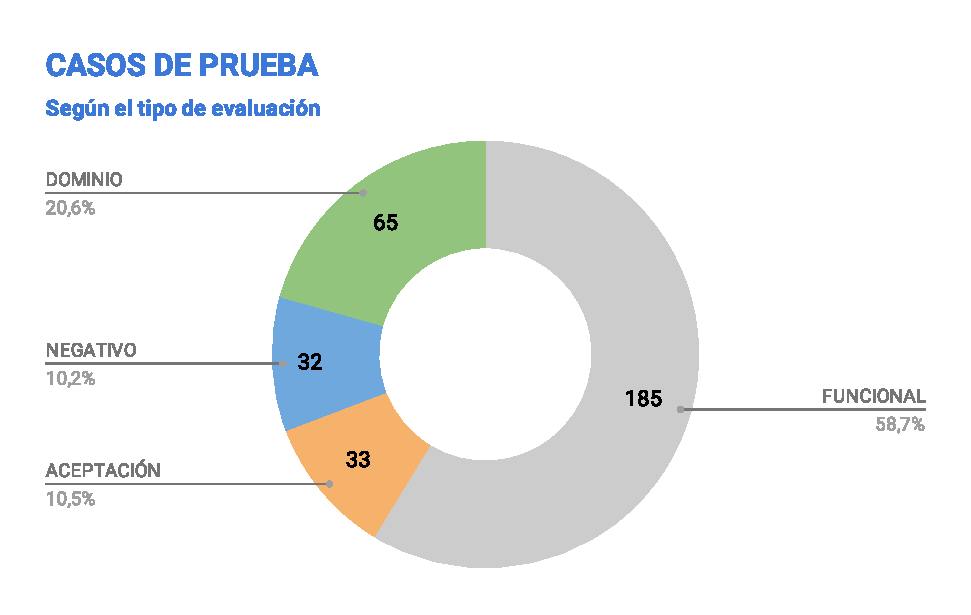
\includegraphics[width=1.0\textwidth]{graphics/tc-tests.eps}
\caption{Casos de Prueba según el tipo de evaluación realizada.}
\label{tc-tests}
\source{Elaboración propia.}
\end{figure}

\begin{figure}
\centering
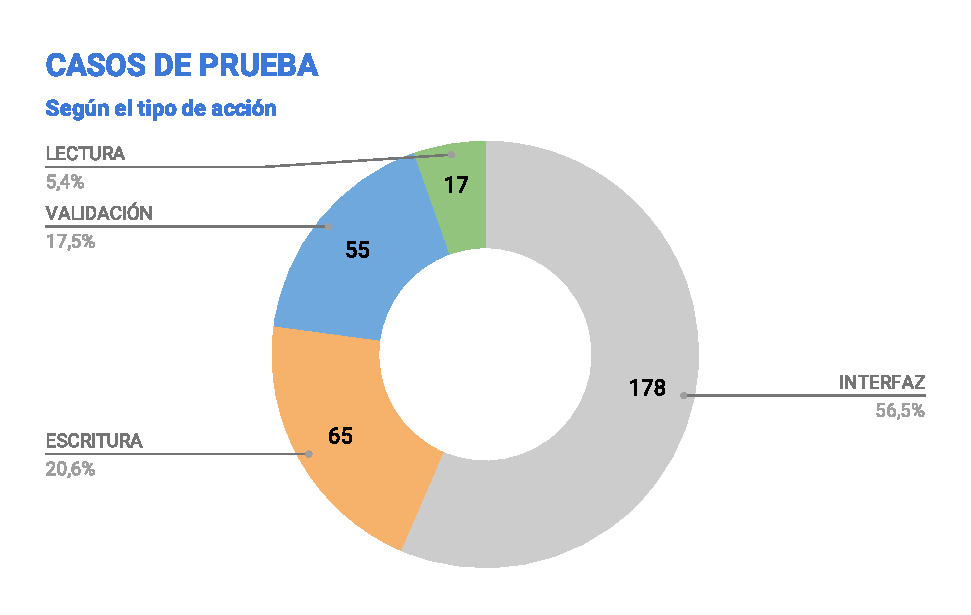
\includegraphics[width=1.0\textwidth]{graphics/tc-type.eps}
\caption{Casos de Prueba según el tipo de acción a evaluar.}
\label{tc-type}
\source{Elaboración propia.}
\end{figure}

